\section{Architecture Overview}

\begin{frame}\frametitle{\secname}\framesubtitle{Section Roadmap}
\begin{itemize}[<+->]
    \item Codebase structure overview.
    \item Views: \texttt{Plugin}, \texttt{Visualization}, \texttt{Audio Engine}.
    \item Stack: \texttt{JUCE} + \texttt{OpenGL}.
    \item Per-view diagrams
    \item Final frame: cross-module connections.
\end{itemize}
\end{frame}

\begin{frame}\frametitle{\secname}\framesubtitle{Plugin}
\begin{columns}[T,totalwidth=\textwidth]
    \column{0.56\textwidth}
    \begin{itemize}[<+->]
        \item Host-facing plugin core and lifecycle.
        \item Main editor and UI composition root.
        \item Centralized parameter model (APVTS).
        \item \textbf{Flow:} host $\rightarrow$ processor $\rightarrow$ parameter/state bridge $\rightarrow$ audio + UI sync.

    \end{itemize}

    \column{0.44\textwidth}
    \only<1>{\textbf{Processor Class Card}}
    \only<2>{\textbf{Editor Class Card}}
    \only<3>{\textbf{Parameter Manager Class Card}}
    \only<4>{\textbf{Atomic GUI State Class Card}}
    \vspace{0.8ex}

    {\centering
    \only<1>{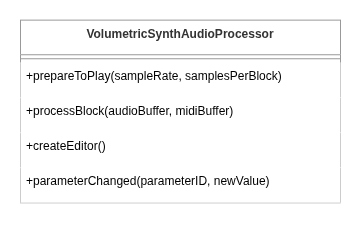
\includegraphics[width=\linewidth,height=0.62\textheight,keepaspectratio]{figures/synth_processor.png}}
    \only<2>{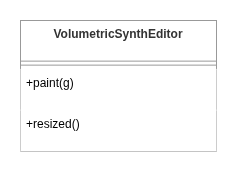
\includegraphics[width=\linewidth,height=0.62\textheight,keepaspectratio]{figures/synth_editor.drawio.png}}
    \only<3>{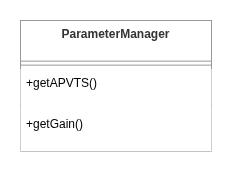
\includegraphics[width=\linewidth,height=0.62\textheight,keepaspectratio]{figures/param_manager.drawio.png}}
    \only<4>{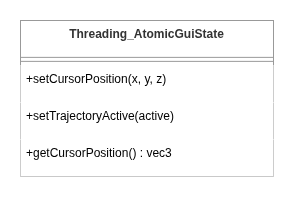
\includegraphics[width=\linewidth,height=0.62\textheight,keepaspectratio]{figures/atomic_gui_state.drawio.png}}
    \par}
\end{columns}
\end{frame}

\begin{frame}\frametitle{\secname}\framesubtitle{Visualization}
\begin{columns}[T,totalwidth=\textwidth]
    \column{0.56\textwidth}
    \begin{itemize}[<+->]
        \item OpenGL cube view renders the 3D interaction space.
        \item Mouse drag drives cube rotation and cursor updates.
        \item Cursor position is normalized and pushed through a lock-free state bridge.
        \item \textbf{Flow:} user gesture $\rightarrow$ 3D view update $\rightarrow$ cursor state $\rightarrow$ DSP.

    \end{itemize}

    \column{0.44\textwidth}
    \only<1>{\textbf{3D View Class Card}}
    \only<2>{\textbf{Interaction Loop Class Card}}
    \only<3>{\textbf{Cursor State Class Card}}
    \only<4>{\textbf{Thread Bridge Class Card}}
    \vspace{0.8ex}

    {\centering
    \only<1>{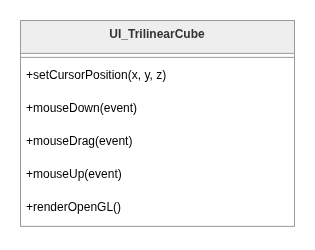
\includegraphics[width=\linewidth,height=0.62\textheight,keepaspectratio]{figures/UI_TrilinearCube.drawio.png}}
    \only<2>{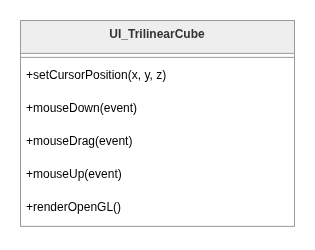
\includegraphics[width=\linewidth,height=0.62\textheight,keepaspectratio]{figures/UI_TrilinearCube.drawio.png}}
    \only<3>{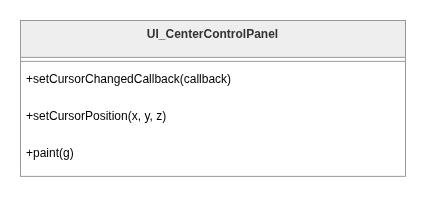
\includegraphics[width=\linewidth,height=0.62\textheight,keepaspectratio]{figures/UI_CenterControlPanel.drawio.png}}
    \only<4>{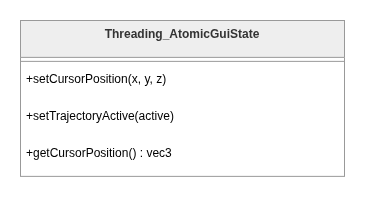
\includegraphics[width=\linewidth,height=0.62\textheight,keepaspectratio]{figures/Threading_AtomicGuiState.drawio.png}}
    \par}
\end{columns}
\end{frame}

\begin{frame}\frametitle{\secname}\framesubtitle{Audio Engine}
\begin{columns}[T,totalwidth=\textwidth]
    \column{0.56\textwidth}
    \begin{itemize}[<+->]
        \item MIDI and audio block orchestration.
        \item Voice allocation and note lifecycle.
        \item Per-voice synthesis signal path.
        \item \textbf{Flow:} MIDI/input $\rightarrow$ voice path $\rightarrow$ oscillator/mixer/envelope $\rightarrow$ output.

    \end{itemize}

    \column{0.44\textwidth}
    \only<1>{\textbf{Synth Engine Class Card}}
    \only<2>{\textbf{Voice Manager Class Card}}
    \only<3>{\textbf{Synth Voice Class Card}}
    \only<4>{\textbf{DSP Stack Class Card}}
    \vspace{0.8ex}

    {\centering
    \only<1>{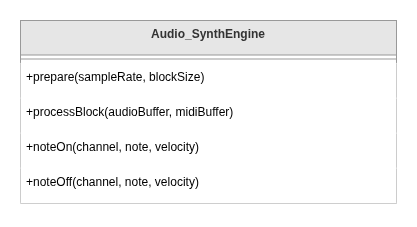
\includegraphics[width=\linewidth,height=0.62\textheight,keepaspectratio]{figures/synth_engine.drawio.png}}
    \only<2>{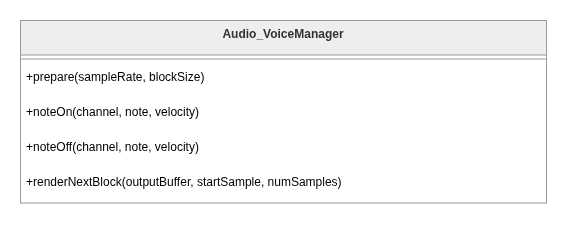
\includegraphics[width=\linewidth,height=0.62\textheight,keepaspectratio]{figures/voice_manager.drawio.png}}
    \only<3>{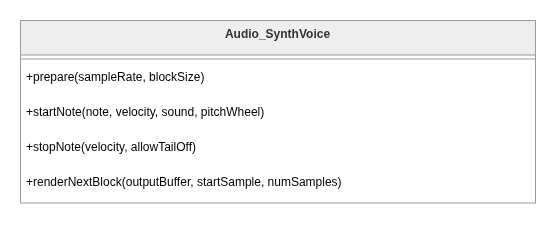
\includegraphics[width=\linewidth,height=0.62\textheight,keepaspectratio]{figures/synth_voice.drawio.png}}
    \only<4>{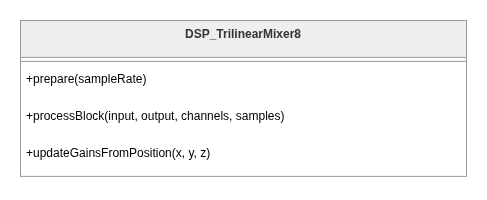
\includegraphics[width=\linewidth,height=0.62\textheight,keepaspectratio]{figures/trilinear_mixer.drawio.png}}
    \par}
\end{columns}
\end{frame}

\begin{frame}\frametitle{\secname}\framesubtitle{End-to-End Integration}
\begin{columns}[T,totalwidth=\textwidth]
    \column{0.56\textwidth}
    \begin{itemize}[<+->]
        \item User interaction enters through the editor layer.
        \item Control and state propagate into real-time paths.
        \item Rendering path flows from engine to voices to DSP output.
        \item \textbf{Flow:} UI $\rightarrow$ control/state bridge $\rightarrow$ processor $\rightarrow$ audio output.
    \end{itemize}

    \column{0.44\textwidth}
    \only<1>{\textbf{System Integration Overview}}
    \only<2>{\textbf{Control Path Focus}}
    \only<3>{\textbf{Processor Coordination Focus}}
    \only<4>{\textbf{Render Pipeline Focus}}
    \vspace{0.8ex}

    {\centering
    \only<1>{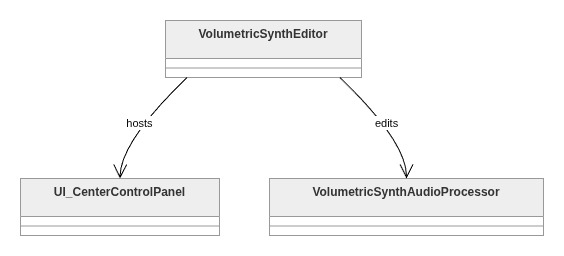
\includegraphics[width=\linewidth,height=0.62\textheight,keepaspectratio]{figures/end2end_1.jpg}}
    \only<2>{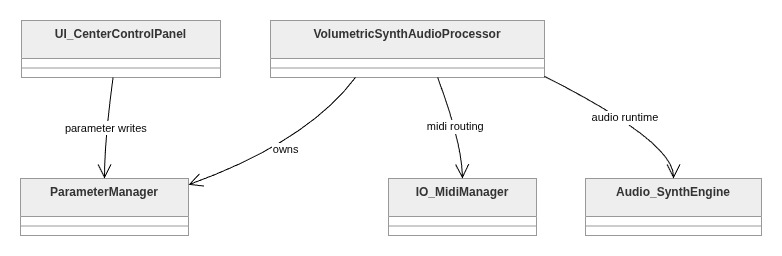
\includegraphics[width=\linewidth,height=0.62\textheight,keepaspectratio]{figures/end2end_2.jpg}}
    \only<3>{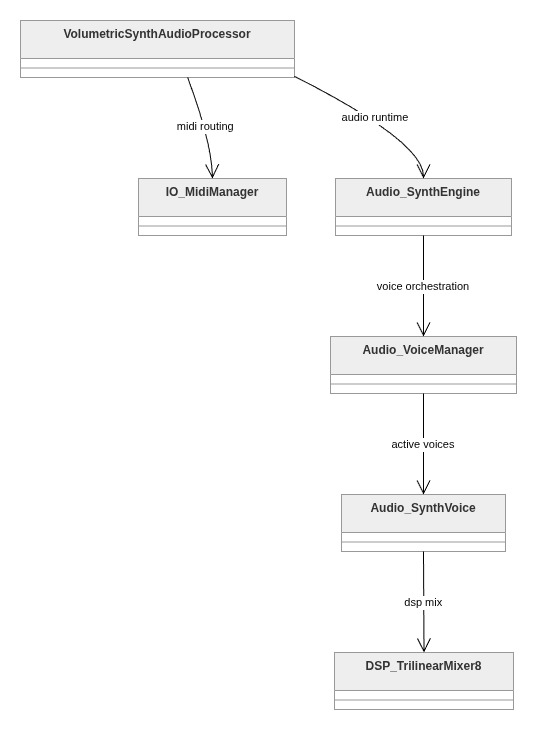
\includegraphics[width=\linewidth,height=0.62\textheight,keepaspectratio]{figures/end2end_3.jpg}}
    \only<4>{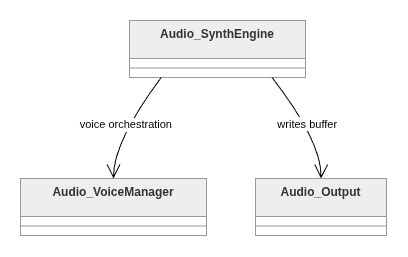
\includegraphics[width=\linewidth,height=0.62\textheight,keepaspectratio]{figures/end2end_4.jpg}}
    \par}
\end{columns}
\end{frame}
